\chapter{Background}

\section{Existing Implementations}

There are several existing technologies and implementations which achieve some of the goals that this project aims to reach. Although there are many which solve a specific problem, there is no application which combines all of the desired aims into one cohesive, accessible, and intuitive system. Below are some of the techniques and existing systems with explanations of how they are used.

\subsection{Ambience Generators}
A popular sound-based method people often use to relax is listening to ambient environments. Users can listen to a curated mix of ambient noises which create a cohesive soundscape. For example, an evening camping trip environment might consist of a sound combination of a campfire, trees blowing in the wind, a distant river and crickets, while a city environment may consist of overlapping chatter, footsteps, car horns and construction noises.

Research has shown that exposure to certain types of ambient sounds can help reduce stress and relax the listener. \cite{song2023effects} found that after listening to nature sounds (water and birds in a forest), participants’ heart rates lowered, and they felt more comfortable and relaxed.

There are many sites which offer many different ambient presets to listen to, such as \textit{soundescape.fm}, \textit{generative.fm}, or \textit{mynoise.net} (see Figure \ref{fig:mynoise}), however, these often do not incorporate melodic or rhythmic instruments or offer any form of real-time collaboration.

\begin{figure}[htb]
    \centering
    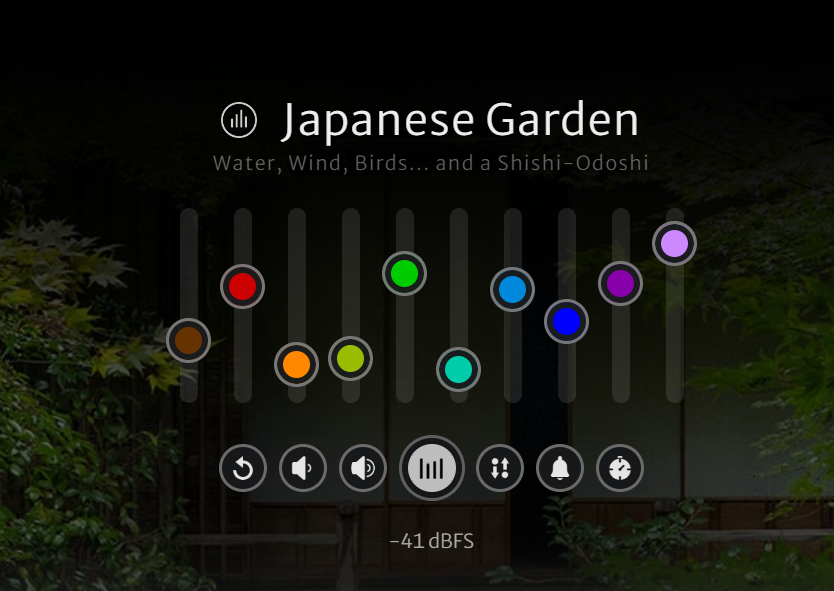
\includegraphics[width=0.5\linewidth]{images/background/mynoise.png}    

    \caption{Screenshot from \textit{mynoise.net}, an ambience generator where users can mix together a number of curated sounds to create a soundscape.}

    \label{fig:mynoise}

\end{figure}

\subsection{Sequencers and Drum Machines}
A sequencer is a common music production tool which typically involves sequencing audio in a loop so that sounds are triggered in a certain pattern. Drum machines are a type of sequencer which are typically limited to short drum or percussion samples, such as kick and snare drums, cymbals, and other percussive sounds like claps or shakers. The main purpose of these is to create drum beats, and there are online tools such as \textit{drumbit.app} (see Figure \ref{fig:drumbit}) or \textit{virtualdrumming.com} which allow for the creation and playback of these patterns. Most tools offer a variety of percussive sounds and typically across 16 time steps, four for each beat in a 4/4 time signature.

\begin{figure}[htb]
    \centering
    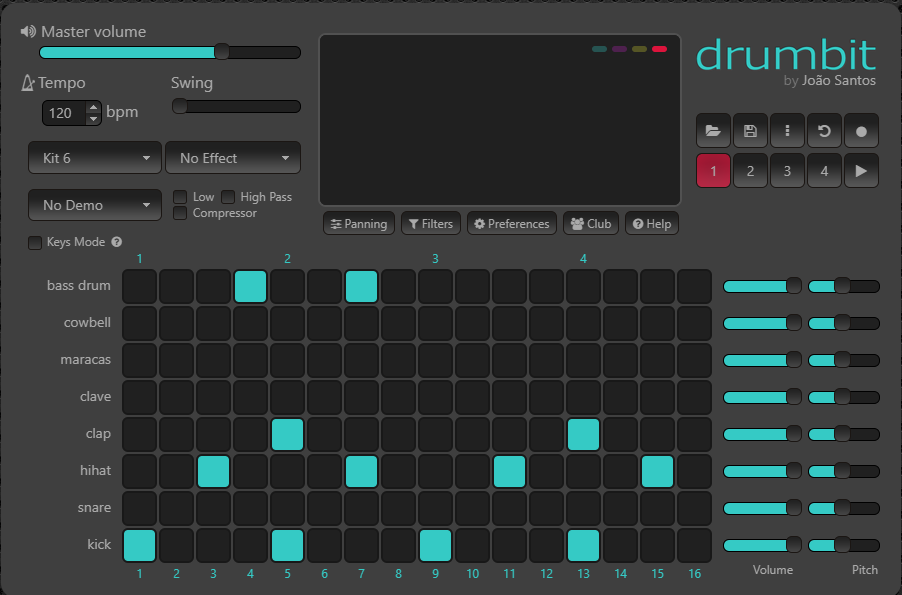
\includegraphics[width=0.5\linewidth]{images/background/drumbit.png}    

    \caption{Screenshot from drumbit.app, a drum machine where users can create a drum pattern by toggling on and off the different drum samples at specified time steps.}

    \label{fig:drumbit}

\end{figure}

Similarly to the ambient sound generators discussed previously, these tools offer plenty of local functionality for their specific purpose (in this case as a drum machine), but do not incorporate instruments or real-time collaboration.

\subsection{Collaborative Music Production and DAWs}
Much of modern music production involves the use of Digital Audio Workstations (DAWs) such as \textit{FLStudio} (see Figure \ref{fig:flstudio}), \textit{Ableton}, or \textit{Reaper}. These applications allow for the recording, editing, and production of music through the use of various methods such as recording live instruments, inputting notes using MIDI controllers, or digitally manipulating sounds using filters and various effects.

\begin{figure}[htb]
    \centering
    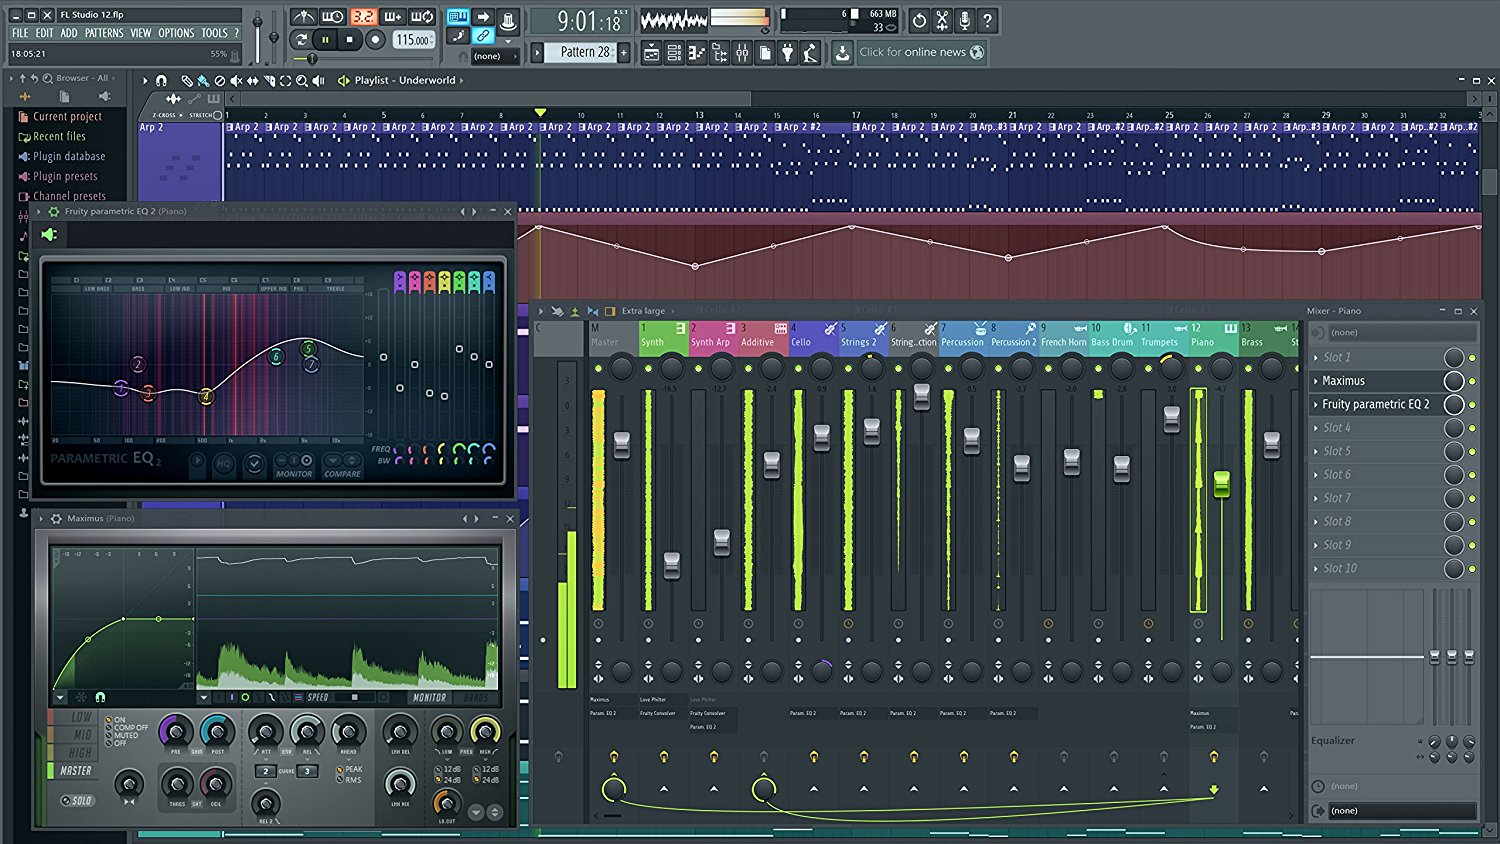
\includegraphics[width=0.5\linewidth]{images/background/flstudio.jpg}    

    \caption{Screenshot from FL Studio, a popular DAW application for producing music.}

    \label{fig:flstudio}

\end{figure}

There are online applications such as \textit{soundtrap.com} (see Figure \ref{fig:soundtrap}), which offer a DAW-like experience through a browser, allowing for collaboration in producing music, however, these tools often require prior music production experience in order to be understood and used effectively. Additionally, the music-making process is usually iterative and finite in nature, as collaboration is done to create a concrete track with a beginning and end. The aim of this project is to create a music-making experience which is accessible for users with no production experience, where music is created in real-time and users can collaborate together to alter how the sound changes as it is being generated.

\begin{figure}[htb]
    \centering
    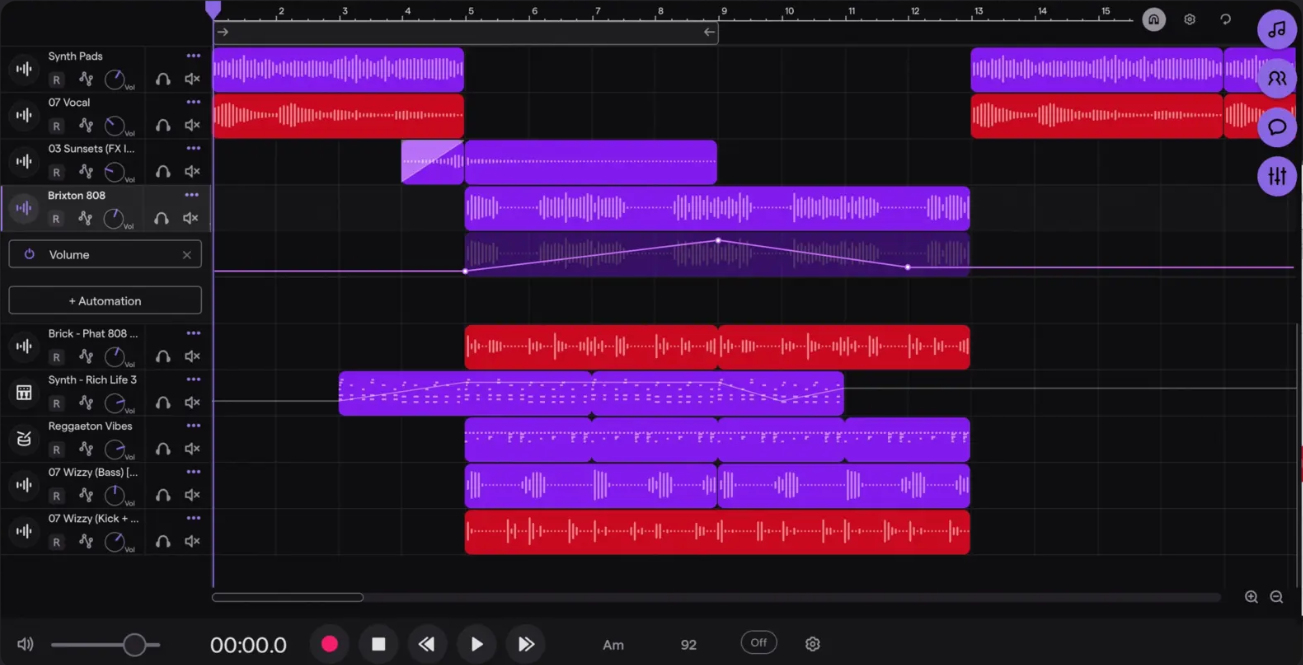
\includegraphics[width=0.5\linewidth]{images/background/soundtrap.png}    

    \caption{Screenshot from soundtrap.com, an online DAW which offers many features as other popular DAWs but in a collaborative online environment.}

    \label{fig:soundtrap}

\end{figure}

\section{Procedurally Generated Music}

Procedurally generated music (sometimes referred to as “adaptive”, “dynamic”, or “interactive” music) generally refers to music which is created algorithmically rather than concretely composed by a person. Typically, this is done through the use of predefined algorithms, parameterisation, and some form of randomisation.

\subsection{Creating Music Algorithmically}
Although randomly generated melodies can be easily achieved by, for example, picking a random piano note every second and playing the result, algorithmically generating convincing music requires a lot more nuisance and a low-level compositional understanding to sound realistic.

A guide for \textit{Procjam} by \cite{procjam} contains information on generating realistic and engaging music by incorporating rules on musical concepts such as repetition, harmonic intervals, and melodic density. Having parameters such as rhythmic density which alter the music generation is a way for users to change the sound as it is being generated.

Commonly found in video games or other interactive entertainment, procedurally generated music can accompany and react in real time to the context or events happening in the game environment. A modern technique called “vertical remixing” is to dynamically swap out instruments to change the musical timbre of the accompanying composition.

\subsection{Implementations}
There are not many online tools which procedurally generate music in real-time. Some sites such as \textit{dopeloop.ai/melody-generator} (see Figure \ref{fig:dopeloop}) or \textit{app.soundgrail.com/melody-generator} offer rudimentary melody creation in various scales, tempos, and instruments, however, neither support real-time generation and playback of those melodies, or allow users to adjust the parameters of the melodies as they are created.

\begin{figure}[htb]
    \centering
    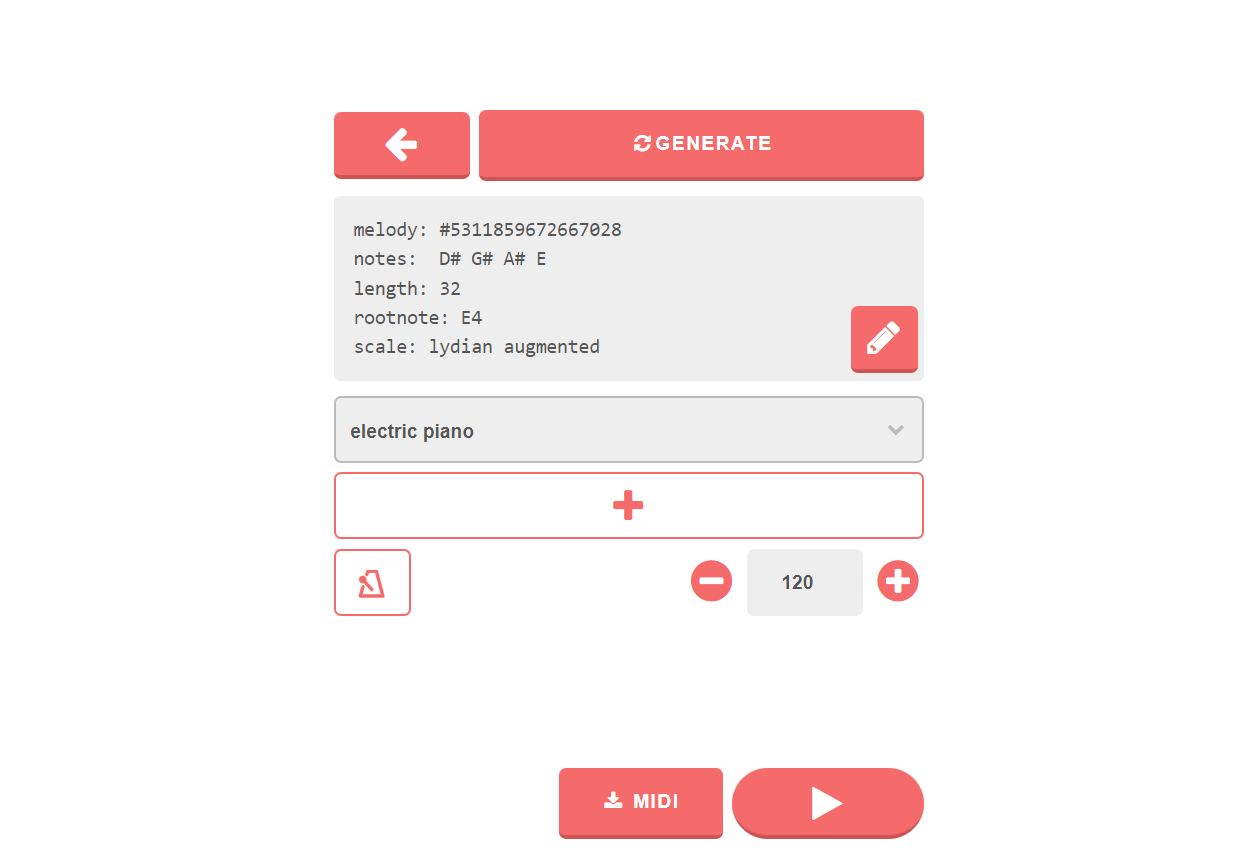
\includegraphics[width=0.5\linewidth]{images/background/dopeloop.png}    

    \caption{Screenshot from dopeloop.ai/melody-generator, a tool to generate and play short melodies in a variety of scales and instruments.}

    \label{fig:dopeloop}

\end{figure}

The design section discusses more on generating music in real-time, in particular the techniques, rules, and algorithms used for this project’s instruments.

\subsection{Psychology of Collaborative Music-Making}
In traditional collaborative music making, there are strong social and psychological factors which contribute to the result, such as the dynamics between musicians, the effectiveness of communication, and the shared goal of the group.
\todo{finish this section}

\section{Consolidating Ideas}
The project will combine aspects and features from each of these categories and consolidate them into one cohesive system which incorporates elements from the categories of music creation covered in this section.
